\documentclass{standalone}
\usepackage{tikz}
\usetikzlibrary{patterns, positioning}
\usepackage[sfdefault]{ClearSans} %% option 'sfdefault' activates Clear Sans as the default text font
\usepackage[T1]{fontenc}

\begin{document}
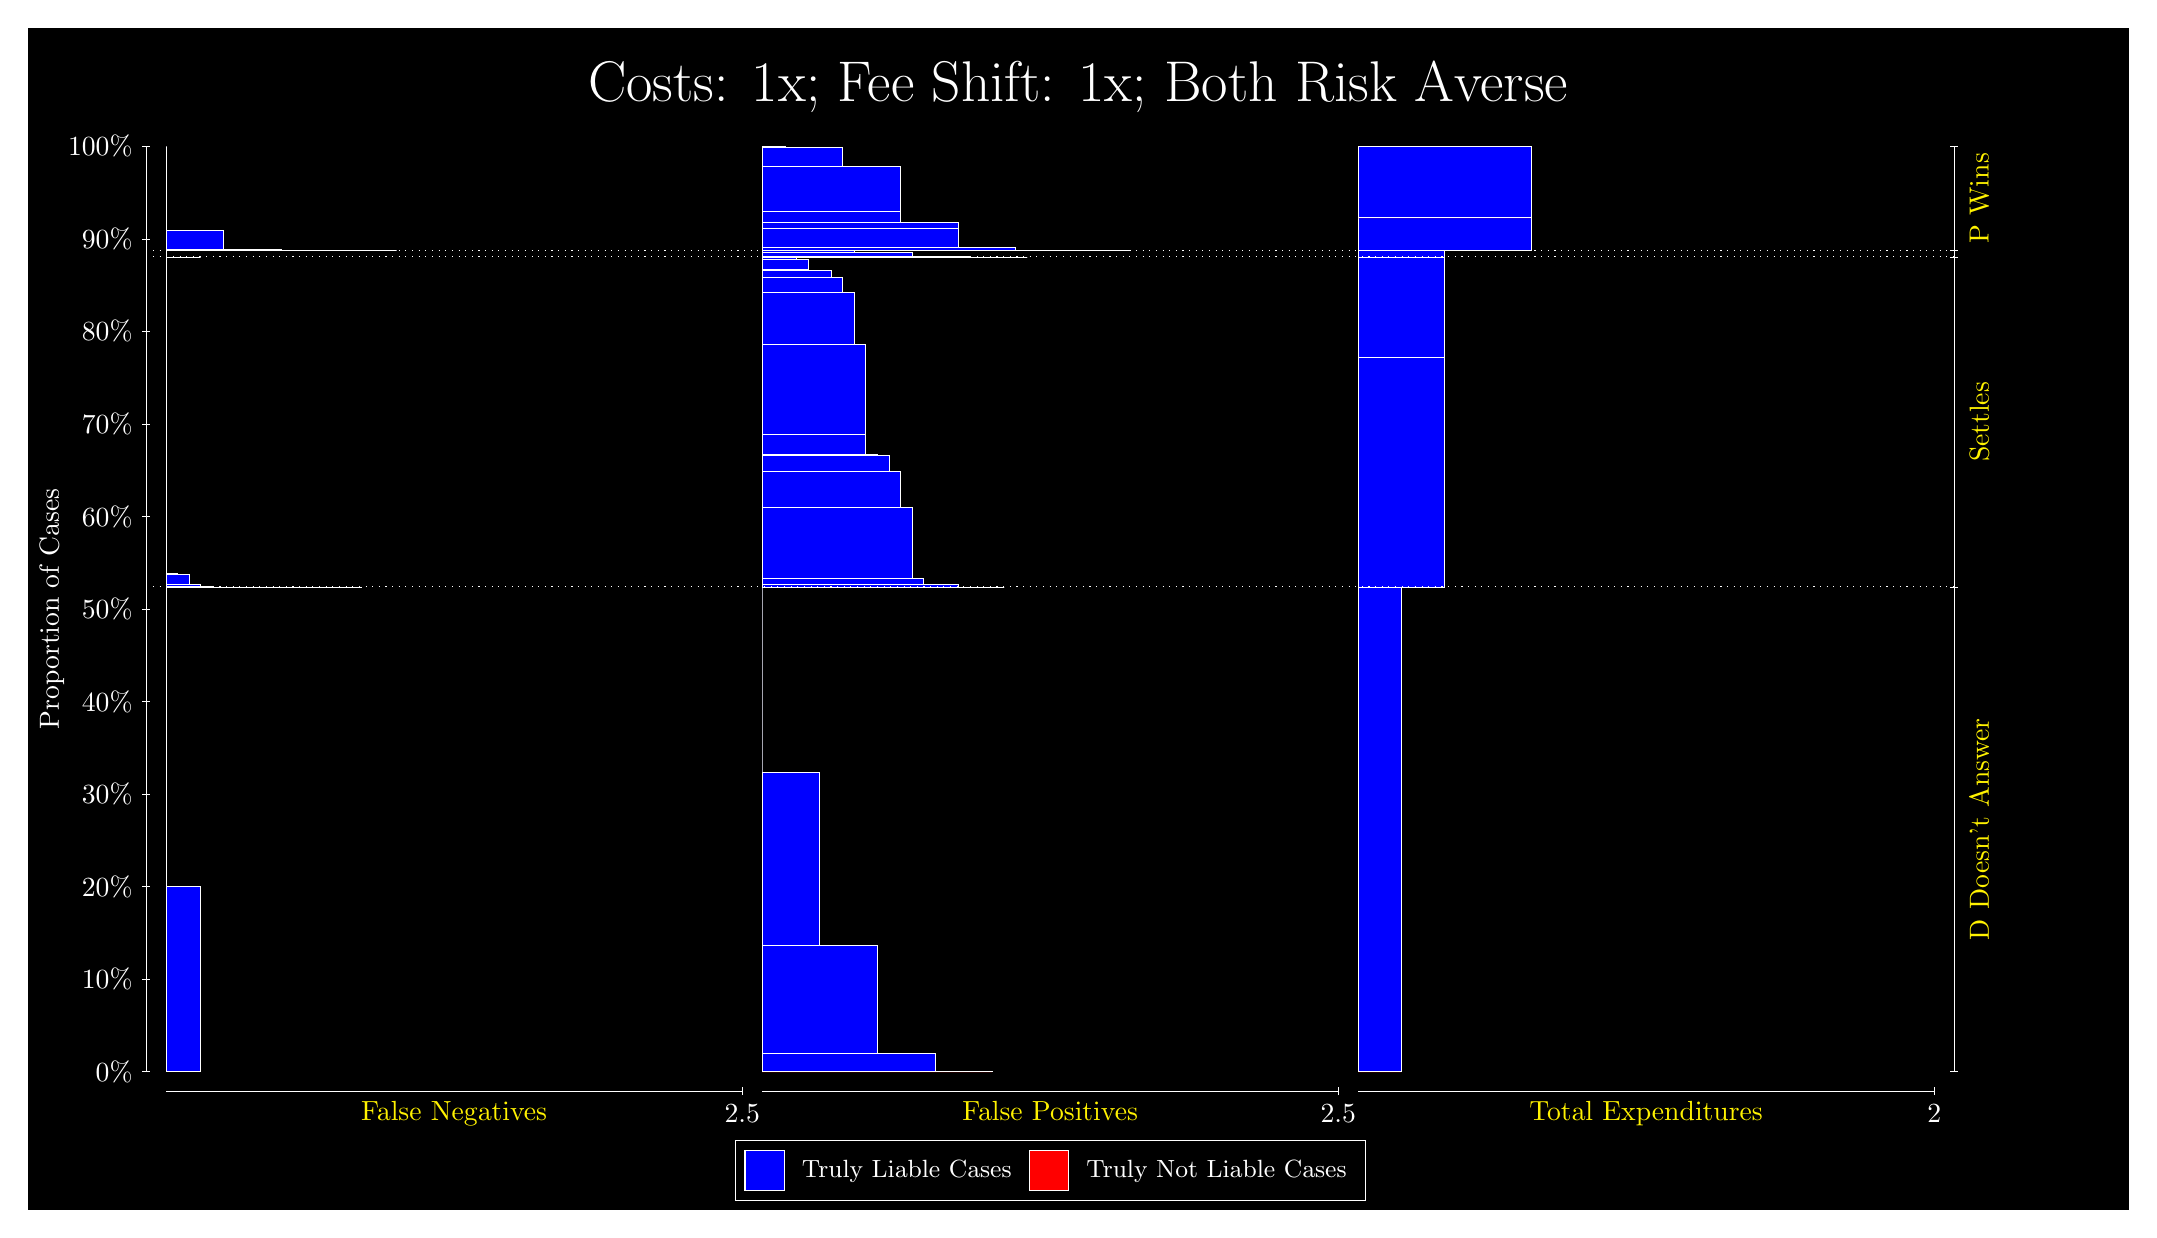
\begin{tikzpicture}
\draw[fill=black] (0,0) rectangle (26.667,15);
\draw[text=white] (0,13.5) rectangle (26.667,15) node[midway] {\huge Costs: 1x; Fee Shift: 1x; Both Risk Averse};
\draw[white, very thin] (1.5,1.75) -- (1.5,13.5);
\node[rotate=90, text=white, anchor=center] at (0.3, 7.625) {Proportion of Cases};
\draw[white, very thin] (1.45,1.75) -- (1.55,1.75);
\node[text=white, anchor=east] at (1.45, 1.75) {0\%};
\draw[white, very thin] (1.45,2.925) -- (1.55,2.925);
\node[text=white, anchor=east] at (1.45, 2.925) {10\%};
\draw[white, very thin] (1.45,4.1) -- (1.55,4.1);
\node[text=white, anchor=east] at (1.45, 4.1) {20\%};
\draw[white, very thin] (1.45,5.275) -- (1.55,5.275);
\node[text=white, anchor=east] at (1.45, 5.275) {30\%};
\draw[white, very thin] (1.45,6.45) -- (1.55,6.45);
\node[text=white, anchor=east] at (1.45, 6.45) {40\%};
\draw[white, very thin] (1.45,7.625) -- (1.55,7.625);
\node[text=white, anchor=east] at (1.45, 7.625) {50\%};
\draw[white, very thin] (1.45,8.8) -- (1.55,8.8);
\node[text=white, anchor=east] at (1.45, 8.8) {60\%};
\draw[white, very thin] (1.45,9.975) -- (1.55,9.975);
\node[text=white, anchor=east] at (1.45, 9.975) {70\%};
\draw[white, very thin] (1.45,11.15) -- (1.55,11.15);
\node[text=white, anchor=east] at (1.45, 11.15) {80\%};
\draw[white, very thin] (1.45,12.325) -- (1.55,12.325);
\node[text=white, anchor=east] at (1.45, 12.325) {90\%};
\draw[white, very thin] (1.45,13.5) -- (1.55,13.5);
\node[text=white, anchor=east] at (1.45, 13.5) {100\%};

\draw[white, very thin] (24.457,1.75) -- (24.457,13.5);
\draw[white, very thin] (24.407,1.75) -- (24.507,1.75);
\node[anchor=west] at (24.407, 1.75) {};
\draw[white, very thin] (24.407,7.9049) -- (24.507,7.9049);
\node[anchor=west] at (24.407, 7.9049) {};
\draw[white, very thin] (24.407,12.096) -- (24.507,12.096);
\node[anchor=west] at (24.407, 12.096) {};
\draw[white, very thin] (24.407,12.181) -- (24.507,12.181);
\node[anchor=west] at (24.407, 12.181) {};
\draw[white, very thin] (24.407,13.5) -- (24.507,13.5);
\node[anchor=west] at (24.407, 13.5) {};

\draw[white, very thin, fill=blue] (1.75,1.75) rectangle (2.1891,4.0985);
\draw[white, very thin, fill=red] (1.75,4.0985) rectangle (1.75,4.0985);
\draw[white, very thin, fill=blue] (1.75,4.0985) rectangle (1.75,7.9049);
\draw[white, very thin, fill=blue] (1.75,7.9049) rectangle (4.2384,7.9049);
\draw[white, very thin, fill=blue] (1.75,7.9049) rectangle (3.6529,7.9049);
\draw[white, very thin, fill=blue] (1.75,7.9049) rectangle (3.5065,7.9049);
\draw[white, very thin, fill=blue] (1.75,7.9049) rectangle (3.3602,7.9049);
\draw[white, very thin, fill=blue] (1.75,7.9049) rectangle (3.0674,7.9049);
\draw[white, very thin, fill=blue] (1.75,7.9049) rectangle (2.921,7.9049);
\draw[white, very thin, fill=blue] (1.75,7.9049) rectangle (2.7746,7.9051);
\draw[white, very thin, fill=blue] (1.75,7.9051) rectangle (2.6283,7.9051);
\draw[white, very thin, fill=blue] (1.75,7.9051) rectangle (2.4819,7.9061);
\draw[white, very thin, fill=blue] (1.75,7.9061) rectangle (2.3355,7.9103);
\draw[white, very thin, fill=blue] (1.75,7.9103) rectangle (2.1891,7.938);
\draw[white, very thin, fill=blue] (1.75,7.938) rectangle (2.0428,8.0612);
\draw[white, very thin, fill=blue] (1.75,8.0612) rectangle (2.0428,8.0712);
\draw[white, very thin, fill=blue] (1.75,8.0712) rectangle (1.8964,8.0717);
\draw[white, very thin, fill=red] (1.75,8.0717) rectangle (1.75,8.0717);
\draw[white, very thin, fill=blue] (1.75,8.0717) rectangle (1.75,12.096);
\draw[white, very thin, fill=blue] (1.75,12.096) rectangle (2.1891,12.096);
\draw[white, very thin, fill=red] (1.75,12.096) rectangle (1.75,12.096);
\draw[white, very thin, fill=blue] (1.75,12.096) rectangle (1.75,12.181);
\draw[white, very thin, fill=blue] (1.75,12.181) rectangle (4.6775,12.181);
\draw[white, very thin, fill=blue] (1.75,12.181) rectangle (3.9457,12.181);
\draw[white, very thin, fill=blue] (1.75,12.181) rectangle (3.2138,12.187);
\draw[white, very thin, fill=blue] (1.75,12.187) rectangle (2.4819,12.432);
\draw[white, very thin, fill=red] (1.75,12.432) rectangle (1.75,12.432);
\draw[white, very thin, fill=blue] (1.75,12.432) rectangle (1.75,13.5);
\draw[white, very thin, fill=red] (9.3189,1.75) rectangle (12.246,1.75);
\draw[white, very thin, fill=blue] (9.3189,1.75) rectangle (12.246,1.7523);
\draw[white, very thin, fill=blue] (9.3189,1.7523) rectangle (11.515,1.9846);
\draw[white, very thin, fill=blue] (9.3189,1.9846) rectangle (10.783,3.3506);
\draw[white, very thin, fill=blue] (9.3189,3.3506) rectangle (10.051,5.5564);
\draw[white, very thin, fill=blue] (9.3189,5.5564) rectangle (9.3189,7.9049);
\draw[white, very thin, fill=red] (9.3189,7.9049) rectangle (12.393,7.9049);
\draw[white, very thin, fill=blue] (9.3189,7.9049) rectangle (12.393,7.9049);
\draw[white, very thin, fill=red] (9.3189,7.9049) rectangle (12.1,7.9049);
\draw[white, very thin, fill=blue] (9.3189,7.9049) rectangle (12.1,7.905);
\draw[white, very thin, fill=red] (9.3189,7.905) rectangle (11.807,7.905);
\draw[white, very thin, fill=blue] (9.3189,7.905) rectangle (11.807,7.9328);
\draw[white, very thin, fill=blue] (9.3189,7.9328) rectangle (11.661,7.9398);
\draw[white, very thin, fill=red] (9.3189,7.9398) rectangle (11.515,7.9398);
\draw[white, very thin, fill=blue] (9.3189,7.9398) rectangle (11.515,7.9405);
\draw[white, very thin, fill=blue] (9.3189,7.9405) rectangle (11.368,8.0118);
\draw[white, very thin, fill=red] (9.3189,8.0118) rectangle (11.222,8.0118);
\draw[white, very thin, fill=blue] (9.3189,8.0118) rectangle (11.222,8.9119);
\draw[white, very thin, fill=blue] (9.3189,8.9119) rectangle (11.075,9.3786);
\draw[white, very thin, fill=blue] (9.3189,9.3786) rectangle (10.929,9.5802);
\draw[white, very thin, fill=blue] (9.3189,9.5802) rectangle (10.783,9.5944);
\draw[white, very thin, fill=blue] (9.3189,9.5944) rectangle (10.636,9.8413);
\draw[white, very thin, fill=red] (9.3189,9.8413) rectangle (10.636,9.8413);
\draw[white, very thin, fill=blue] (9.3189,9.8413) rectangle (10.636,10.992);
\draw[white, very thin, fill=blue] (9.3189,10.992) rectangle (10.49,11.645);
\draw[white, very thin, fill=blue] (9.3189,11.645) rectangle (10.344,11.832);
\draw[white, very thin, fill=blue] (9.3189,11.832) rectangle (10.197,11.929);
\draw[white, very thin, fill=blue] (9.3189,11.929) rectangle (10.051,11.93);
\draw[white, very thin, fill=blue] (9.3189,11.93) rectangle (9.9044,11.94);
\draw[white, very thin, fill=blue] (9.3189,11.94) rectangle (9.9044,12.063);
\draw[white, very thin, fill=blue] (9.3189,12.063) rectangle (9.758,12.091);
\draw[white, very thin, fill=blue] (9.3189,12.091) rectangle (9.6116,12.095);
\draw[white, very thin, fill=blue] (9.3189,12.095) rectangle (9.4652,12.096);
\draw[white, very thin, fill=blue] (9.3189,12.096) rectangle (9.3189,12.096);
\draw[white, very thin, fill=red] (9.3189,12.096) rectangle (12.686,12.096);
\draw[white, very thin, fill=blue] (9.3189,12.096) rectangle (12.686,12.096);
\draw[white, very thin, fill=blue] (9.3189,12.096) rectangle (11.954,12.098);
\draw[white, very thin, fill=blue] (9.3189,12.098) rectangle (11.222,12.151);
\draw[white, very thin, fill=blue] (9.3189,12.151) rectangle (10.49,12.18);
\draw[white, very thin, fill=blue] (9.3189,12.18) rectangle (9.758,12.181);
\draw[white, very thin, fill=red] (9.3189,12.181) rectangle (14.003,12.181);
\draw[white, very thin, fill=blue] (9.3189,12.181) rectangle (14.003,12.181);
\draw[white, very thin, fill=red] (9.3189,12.181) rectangle (13.271,12.181);
\draw[white, very thin, fill=blue] (9.3189,12.181) rectangle (13.271,12.181);
\draw[white, very thin, fill=red] (9.3189,12.181) rectangle (12.539,12.181);
\draw[white, very thin, fill=blue] (9.3189,12.181) rectangle (12.539,12.213);
\draw[white, very thin, fill=blue] (9.3189,12.213) rectangle (11.807,12.459);
\draw[white, very thin, fill=red] (9.3189,12.459) rectangle (11.807,12.459);
\draw[white, very thin, fill=blue] (9.3189,12.459) rectangle (11.807,12.541);
\draw[white, very thin, fill=blue] (9.3189,12.541) rectangle (11.075,12.675);
\draw[white, very thin, fill=red] (9.3189,12.675) rectangle (11.075,12.675);
\draw[white, very thin, fill=blue] (9.3189,12.675) rectangle (11.075,13.248);
\draw[white, very thin, fill=blue] (9.3189,13.248) rectangle (10.344,13.249);
\draw[white, very thin, fill=blue] (9.3189,13.249) rectangle (10.344,13.494);
\draw[white, very thin, fill=blue] (9.3189,13.494) rectangle (9.6116,13.494);
\draw[white, very thin, fill=blue] (9.3189,13.494) rectangle (9.6116,13.5);
\draw[white, very thin, fill=blue] (9.3189,13.5) rectangle (9.3189,13.5);
\draw[white, very thin, fill=red] (16.888,1.75) rectangle (17.437,1.75);
\draw[white, very thin, fill=blue] (16.888,1.75) rectangle (17.437,7.9049);
\draw[white, very thin, fill=red] (16.888,7.9049) rectangle (17.986,7.9049);
\draw[white, very thin, fill=blue] (16.888,7.9049) rectangle (17.986,10.822);
\draw[white, very thin, fill=red] (16.888,10.822) rectangle (17.986,10.822);
\draw[white, very thin, fill=blue] (16.888,10.822) rectangle (17.986,12.096);
\draw[white, very thin, fill=red] (16.888,12.096) rectangle (17.986,12.096);
\draw[white, very thin, fill=blue] (16.888,12.096) rectangle (17.986,12.181);
\draw[white, very thin, fill=red] (16.888,12.181) rectangle (19.083,12.181);
\draw[white, very thin, fill=blue] (16.888,12.181) rectangle (19.083,12.593);
\draw[white, very thin, fill=red] (16.888,12.593) rectangle (19.083,12.593);
\draw[white, very thin, fill=blue] (16.888,12.593) rectangle (19.083,13.5);
\draw[white, dotted] (1.5,7.9049) -- (24.457,7.9049);
\draw[white, dotted] (1.5,12.096) -- (24.457,12.096);
\draw[white, dotted] (1.5,12.181) -- (24.457,12.181);
\draw[white, very thin] (1.75,1.5) -- (9.0689,1.5);
\node[text=yellow, anchor=north] at (5.4094, 1.5) {False Negatives};
\draw[white, very thin] (9.0689,1.45) -- (9.0689,1.55);
\node[text=white, anchor=north] at (9.0689, 1.45) {2.5};

\draw[white, very thin] (9.3189,1.5) -- (16.638,1.5);
\node[text=yellow, anchor=north] at (12.978, 1.5) {False Positives};
\draw[white, very thin] (16.638,1.45) -- (16.638,1.55);
\node[text=white, anchor=north] at (16.638, 1.45) {2.5};

\draw[white, very thin] (16.888,1.5) -- (24.207,1.5);
\node[text=yellow, anchor=north] at (20.547, 1.5) {Total Expenditures};
\draw[white, very thin] (24.207,1.45) -- (24.207,1.55);
\node[text=white, anchor=north] at (24.207, 1.45) {2};

\node[text=yellow, centered, rotate=90] at (24.777, 4.8274) {D Doesn't Answer};
\node[text=yellow, centered, rotate=90] at (24.777, 10) {Settles};

\node[text=yellow, centered, rotate=90] at (24.777, 12.84) {P Wins};

\draw (12.978300999999998,1.5) node[draw=none] (baseCoordinate) {};
\begin{scope}[align=center]
        \matrix[scale=0.5, draw=white, below=0.5cm of baseCoordinate, nodes={draw}, column sep=0.1cm]{
            \node[rectangle, draw, minimum width=0.5cm, minimum height=0.5cm, fill=blue] {}; &
            \node[draw=none, font=\small, text=white] (B) {Truly Liable Cases}; &
            \node[rectangle, draw, minimum width=0.5cm, minimum height=0.5cm, fill=red] {}; &
            \node[draw=none, font=\small, text=white] (B) {Truly Not Liable Cases}; \\
            };
\end{scope}

\end{tikzpicture}
\end{document}